\documentclass[]{report}

\voffset=-1.5cm
\oddsidemargin=0.0cm
\textwidth = 480pt

\usepackage{framed}
\usepackage{subfiles}
\usepackage{enumerate}
\usepackage{graphics}
\usepackage{newlfont}
\usepackage{eurosym}
\usepackage{amsmath,amsthm,amsfonts}
\usepackage{amsmath}
\usepackage{color}
\usepackage{amssymb}
\usepackage{multicol}
\usepackage[dvipsnames]{xcolor}
\usepackage{graphicx}
\begin{document}
	


\chapter{Session 7}

%------------------------------------%

\section*{Session 07:Sequences and Series}
\begin{itemize}
\item[7A.1] Sequences
\item[7A.2] Induction
\item[7A.3] Series and the Sigma Notation
\end{itemize}

\subsection*{Recurrence Relations(7.1.1)}



$u_1 = 2$
$u_2 = u_1 + 3 = 2 +3 = 5$
$u_3 = u_2 + 3 = 5+ 3 = 8$
Airthmetic Progression


\subsection*{Proof by Induction(7.2.2)}
\begin{itemize}
\item[Step 1] Base case
\item[Step 2] Induction hypothesis
\item[Step 3] Induction step
\end{itemize}



\subsection*{Series and Sigma Notation(7.2.3)}




Say which of the set the following numbers belong to.

If they belong to more than one of these sets, give all the sets.

$\sqrt{2}$
$\frac{3}{7}$

%------------------------------------------------------



\subsection*{Section 8 Exercises}
\begin{itemize}
\item $8^{\frac{1}{3}}$ Recall $a^{\frac{b}{c}} = a^{\frac{b}{c}}$
\item
\item
\end{itemize}



%------------------------------------%




%------------------------------------%
\subsection{Sequence and Series and Proof by Induction}


\[\sum^{n}_{i=1} (n^2) \]


\subsection*{Question 1}

(b) Express the following hexadecimal number as a decimal number: (A32.8)16.
[3]
(c) Convert the following decimal number into base 2, showing all your working:
$(253)_{10}$. [2]
(d) Express the recurring decimal $0.4242424\ldots$
as a rational number in its simplest
form. [2]


%---------------------------------------%
\subsection*{Question 7}
%2002 Question 7
Let S be a set and let R be a relation on S
Explain what it means to say thet $\mathcal{R}$ is

\begin{itemize}
	\item[(i)] reflexive
	\item[(ii)] symmetrix
	\item[(iii)] anti-symmetric
	\item[(iv)] Transitive
\end{itemize}


\subsection{Question 10}

(a) Given the following adjacency matrices A and B where
A =

1 0 1
0 1 2
1 2 0

,B =

1 2 0
2 0 1
0 1 1

%MAKE NO

%--------------------------------------------%

(i) Say whether or not the graphs they represent are isomorphic.
(ii) Calculate A2 and A4 and say what information each gives about the graph
corresponding to A. [6]
(b) (i) Write down the augmented matrix for the following system of equations.

\[2x + y - z = 2\]
\[x - y + z = 4\]
\[x + 2y + 2z = 10\]
(ii) Use Gaussian elimination to solve the system. [4]


%--------------------------------------------%
\newpage
\chapter{Session 9}
\section{Probability and Counting}

% 2007 Q8
Given S is the set of all 5 digit binary strings, E is the set of a 5 digit
binary strings beginning with a 1 and F is the set of all 5 digit binary strings ending
with two zeroes.
\begin{itemize}
\item[(a)] Find the cardinality of S, E and F.
\item[(b)] Draw a Venn diagram to show the relationship between the sets S, E and F.
\item[(c)]Show the relevant number of elements in each region of your diagram.
\end{itemize}
%-------------------------------------------------------------------------%
\newpage

\textbf{Three Steps}
\begin{description}
\item[Step 1]
\item[Step 2]
\item[Step 3]
\end{description}


{Proof by Induction}

Let the summation $s_n$ be defined as follows:
\[s_n = 1 + 3 + 5 + \ldots + (2n - 1) \qquad \mbox{for n }\in \mathbb{Z}^{+}\]

Use the method of induction to prove that $s_n = n^2$ for all $n \geq 1$.


%------------------------------------------- %


%------------------------- %
% Section 1
\subsection{Axioms of Probability}

The Axioms of Probability

\begin{itemize}
\item The probability of a certain event is 1.
\item The probability of an impossible event is 0.
\item 
\end{itemize}
%------------------------- %
%-------------------------- %
\section*{Session 09: Probability}
\begin{itemize}
\item[9A.1] Counting Methods
\item[9A.2] Counting using Sets
\item[9A.3] Probability
\item[9A.4] Independent Events
\end{itemize}
\begin{itemize}
\item[9B.1] 


%-----------------------------------------------------%







%-----------------------------------------------------%



\section*{Question 10}

\subsection*{Session 10: Matrices and Systems of Equations}
\begin{itemize}
\item[10A.1] Dimensions of a Matrix
\item[10A.2] Matrix Multiplication
\item[10A.3] Matrix Calculations
\item[10A.4] 
\end{itemize}

\begin{itemize}
\item[10B.1] Systems of Equations
\item[10B.2] Expression Systems of Equations as Matrices
\item[10B.3] Augmented Matrices
\item[10B.4] Guassian Elimination
\end{itemize}
%-----------------------------------%
\subsection*{Question 10A}

Say what information the first row of the matrix contains.
Find the number of edges of G.


Write doen the augmented matrix for the following system of equations.
x+y+2z=7
2x+y+3z =11
x-27+5z=4


Use Gaussian elimination to solve the system.


\section{Matrices}

What are the dimensions of the following matrix


\[ \left(
\begin{array}{cc}
a_1 & a_2 \\ 
b_1 & b_2
\end{array} \right)\left(
\begin{array}{cc}
c_1 & d_1 \\ 
c_2 & d_2
\end{array} \right) = \left(
\begin{array}{cc}
(a_1 \times c_1) + (a_2 \times c_2) & (a_1 \times d_1) + (a_2 \times d_2) \\ 
(b_1 \times c_1) + (b_2 \times c_2) & (b_1 \times d_1) + (b_2 \times d_2)
\end{array} \right) \]

\bigskip
\large{
\[ \left(
\begin{array}{cc}
1 & 3 \\ 
0 & 2
\end{array} \right)\left(
\begin{array}{cc}
1 & 2 \\ 
4 & 1
\end{array} \right) = \left(
\begin{array}{cc}
(1 \times 1) + (3 \times 4) & (1 \times 2) + (3 \times 1) \\ 
(0 \times 4) + (2 \times 4) & (0 \times 2) + (2 \times 1)
\end{array} \right) = \left(
\begin{array}{cc}
14 & 5 \\ 
8 & 2
\end{array} \right) \]
}

\[ \left(
\left(
\begin{array}{cc}
1 & 2 \\ 
4 & 1
\end{array} \right)
\begin{array}{cc}
1 & 3 \\ 
0 & 2
\end{array} \right) = ? \]

%=====================================================================%
\subsection*{Question 3}
%2003

\begin{itemize}
\item[(a)] Let n be an element of the set $\{10, 11, 12, 13, 14, 15, 16, 17, 18, 19\}$,
and p and q be the propositions:
\[p : n \mbox{ is odd},   q : n < 15\]. Draw up truth tables for the following statements and find the values of n for
which they are true:
\begin{itemize}
\item[(i)] $ p \vee \neg q$ 
\item[(ii)] $\neg p \wedge q$
\end{itemize}
\item[(b)] Use truth tables to find a statement that is logically equivalent to $\neg p \rightarrow q$.
\end{itemize}

%--------------------- %
% - 1.2 2010 
\begin{enumerate}[(i)]
\item
\end{enumerate}
%=====================================================================%
\subsection*{Question 4}
Let $S$ be the set of all 4 bit binary strings. The function $f : S \rightarrow Z$
is defined by the rule:
\[f(x) = \mbox{ the number of zeros in x} \] for each binary string $x \in S$.
Find:
\begin{itemize}
\item[(a)] (4 Marks) Answer the following questions
\begin{itemize}
\item[(i)] the number of elements in the domain
\item[(ii)] f(1010)
\item[(iii)] the set of pre-images of 1
\item[(iv)] the range of f. 
\end{itemize}
\item[(b)] (2 Marks) Decide whether the function $f$, as defined above, has either the one to one or
the onto property, justifying your answers. 
\item[(c)] (2 Marks) State the condition to be satisfied by a function $f : X \rightarrow Y$ for it to have an
inverse function $f^{-1} : Y \rightarrow X$.
\item[(d)] (2 Marks) Define the inverse functions for each of the following:
\end{itemize}
%---------------------------------------------------------%
%\section*{Question 5}
%
%\begin{figure}
%\centering
%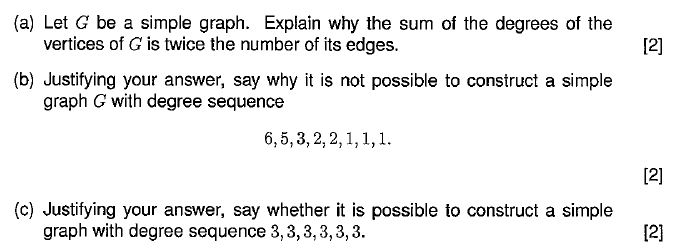
\includegraphics[width=0.7\linewidth]{GraphTheoryQuestion2012}
%
%\end{figure}


%----------------------------------------------------------------%
\newpage
\section*{Question 6}
% 2007 Q8
Given a flock of chickens, between any two chickens one of them is
dominant. A relation, R, is defined between chicken x and chicken y as xRy if x is
dominant over y. This gives what is known as a pecking order to the flock. Home
Farm has 5 chickens: Amy, Beth, Carol, Daisy and Eve, with the following relations:

\begin{itemize}
\item Amy is dominant over Beth and Carol
\item Beth is dominant over Eve and Carol
\item Carol is dominant over Eve and Daisy
\item Daisy is dominant over Eve, Amy and Beth
\item Eve is dominant over Amy.
\end{itemize}

\newpage
\section*{Question 6}
% Digraphs and Relations
% http://staff.scem.uws.edu.au/cgi-bin/cgiwrap/zhuhan/dmath/dm_readall.cgi?page=20

Let $A=\{0,1,2\}$ and $R=\{ (0,0),(0,1),(0,2),(1,1), (1,2), (2,2)\}$
and $S=\{(0,0),(1,1),(2,2)\}$ be 2 relations on A. Show that

\begin{itemize}
\item[(i)] R is a partial order relation.
\item[(ii)] S is an equivalence relation.
\end{itemize}
%---------------------------------------------------------------------------%

%2002 Question 7
Let S be a set and let R be a relation on S
Explain what it means to say thet $\mathcal{R}$ is

\begin{itemize}
\item[(i)] reflexive
\item[(ii)] symmetrix
\item[(iii)] anti-symmetric
\item[(iv)] Transitive
%---------------------------------------------------------------------------%



\end{itemize}
% TREES
\newpage
\section*{Question 8}
%\noindent \textbf{(Part A : Spanning Trees -  5 Marks) }\\
%\begin{figure}[h!]
%\centering
%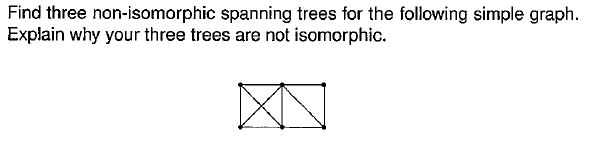
\includegraphics[width=1.11\linewidth]{TreesQuestion2012}
%\end{figure}

%Question 8A
%\begin{enumerate}
%\item How many edges are in the spanning tree $T$ ?
%\item What is the sum of the degree sequence of $T$?
%\item Write down all the possible degree sequences for the spanning tree $T$.
%\end{enumerate}
%---------------------------------------------------------------------------%


\noindent \textbf{(Part B :Binary Search Trees -  5 Marks) }\\
Suppose a database, comprised of 30,000 internal nodes, is structured as a Binary Search Tree.

\begin{enumerate}[(i)]
\item What is the Key of the Root node?
\item What are the keys of the nodes at level 1?
\item For the nodes at level 1, how many subtrees are there?
%\item State which nodes are in the substrees of the level 1 nodes?
\item How many nodes are the between the root (level 0) and level 4. ]
%(Hint: use a summation theorem mentioned in session 7
\item What is the maximum number of searchs in this database?
\end{enumerate}

%============================================================================%

\section*{ Question 9 }
Given S is the set of all 5 digit binary strings, E is the set of a 5 digit
binary strings beginning with a 1 and F is the set of all 5 digit binary strings ending
with two zeroes.
\begin{itemize}
\item[(a)] Find the cardinality of S, E and F.
\item[(b)] Draw a Venn diagram to show the relationship between the sets S, E and F.
Show the relevant number of elements in each region of your diagram.
\end{itemize}

\begin{itemize}
\item A college teaches courses in the following subjects areas: mathematics, computing and statistics.
\item Students in the college may choose their courses from these three subject areas.
\item Students are not obliged to take courses from these three subject areas, and may instead take courses in other subject areas. 
\item  Let the subject areas be represented by the letters \textbf{M} for mathematics, \textbf{C} for computing and \textbf{S} for statistics. \item Draw a labelled Venn diagram showing the areas \textbf{M}, \textbf{C}, and \textbf{S} in such a way as to represent the students studying at the college. \item On your diagram show the number of students studying in each region of the Venn diagram.
%===================%
\begin{itemize}
\item Currently 600
students are enrolled in the college. 
\item 300 students are taking mathematics courses.
\item 120 student are taking statistics courses.
\item 380 students are taking computing courses. 
\item 40 students study courses from all three subject
areas. 
\item 200 mathematics students are taking computing courses as well. \item 60 computing students
are also takings statistics courses. \item  70 statistics students are also taking mathematics course.
\end{itemize}
\end{itemize}

%==============%
\begin{itemize}
\item[(i)] How many students study none of these courses at all?
\item[(ii)] How many students are taking mathematics courses but not computing or statistics courses.
\item[(iii)] How many students study courses from precisely two of these subject
areas?

\end{itemize}
\newpage
%===========================================================%
\section*{Question 10}
%%--------------------------------------------%
%\noindent \textbf{Part A : Matrix Operations - 4 Marks}\\ 
%\begin{figure}[h!]
%\centering
%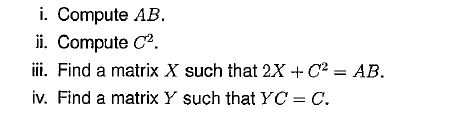
\includegraphics[width=1.11\linewidth]{MatrixQuestion2012}
%
%\end{figure}


%--------------------------------------------%
\noindent \textbf{Part B : Gaussian Elimination - 5 Marks}\\ 
\begin{itemize}
\item[(i)] Say whether or not the graphs they represent are isomorphic.
\item[(ii)] Calculate $A^2$ and $A^4$ and say what information each gives about the graph
corresponding to A. [6]
\end{itemize}
%===========================================%
\begin{itemize}
\item[(i)] Write down the augmented matrix for the following system of equations.
\[2x + y - z = 2\]
\[x - y + z = 4\]
\[x + 2y + 2z = 10\]
\item[(ii)] Use Gaussian elimination to solve the system. 
\end{itemize}
%=========================================================================================== %


%-------------------------------------------------------------------------%
\newpage

\end{document}
